\chapter{Cahn--Hilliard demo}
\label{chap:cahn-hilliard}

\begin{quote}
Spec dir:
\passthrough{\lstinline!specs/2026-05-03-phase-12-cahn-hilliard/!}.
Version: \passthrough{\lstinline!0.12.0!}.
\end{quote}

\subsection{What this gives you}\label{phase12-what}

A real, scientifically meaningful end-to-end example that exercises
the layered abstractions delivered in Phases 1--11. The Cahn--Hilliard
(CH) equation
\[
\partial_t\psi \;=\; M\,\nabla^2\!\Big(\tfrac{\delta F}{\delta \psi}\Big),
\qquad
F[\psi] \;=\; \int\!\Big[-\tfrac12\psi^2 + \tfrac14\psi^4 + \tfrac{\kappa}{2}|\nabla\psi|^2\Big]\,\dd V,
\]
is the canonical model of binary-alloy phase separation. Starting from
a small random fluctuation around the unstable mean \(\bar\psi=0\), the
system spinodally decomposes into two phases at \(\psi\approx\pm 1\),
sharpens the interfaces, then enters a coarsening regime in which the
typical domain size grows as \(R(t)\sim t^{1/3}\) (Bray's
classical-coarsening scaling). The demo reproduces this sequence.

The implementation lives in
\href{../../../examples/cahn_hilliard.cpp}{\passthrough{\lstinline!examples/cahn\_hilliard.cpp!}}
with the CH right-hand side and energy diagnostics factored into
\href{../../../examples/common/cahn_hilliard.hpp}{\passthrough{\lstinline!examples/common/cahn\_hilliard.hpp!}}
so the same code is exercised by the Phase 12 acceptance test
\href{../../../test/cahn_hilliard_test.cpp}{\passthrough{\lstinline!test/cahn\_hilliard\_test.cpp!}}.

\subsection{Free-energy form and variational
derivative}\label{phase12-energy}

The free energy is the standard Landau double-well + gradient term:
\[
f_{\text{bulk}}(\psi) \;=\; -\tfrac12\psi^2 + \tfrac14\psi^4,
\qquad
f_{\text{grad}}(\nabla\psi) \;=\; \tfrac{\kappa}{2}|\nabla\psi|^2.
\]
The bulk has minima at \(\psi=\pm 1\) (the equilibrium phases) and a
local maximum at \(\psi=0\) (the spinodal point). The gradient term
penalizes interfaces and sets their characteristic width
\(\xi\sim\sqrt{\kappa}\).

The variational derivative is supplied in closed form (no automatic
differentiation):
\[
\mu \;:=\; \frac{\delta F}{\delta \psi} \;=\; f_{\text{bulk}}'(\psi) - \kappa\nabla^2\psi
\;=\; -\psi + \psi^3 - \kappa\nabla^2\psi.
\]
Conservative dynamics follows model B:
\[
\partial_t\psi \;=\; M\nabla^2\mu \;=\; M\nabla^2\big(-\psi + \psi^3 - \kappa\nabla^2\psi\big).
\]
The right-hand side requires only Phase 1's
\passthrough{\lstinline!diff::laplacian!}, applied twice per
evaluation (once for \(\nabla^2\psi\), once for the outer
\(\nabla^2\mu\)).

\subsection{Discretization and stability
budget}\label{phase12-stability}

The demo runs on a periodic cubic Cartesian grid with
\(\Delta x = 1\) and the Phase 1 default 2nd-order central-difference
Laplacian. Time stepping is the classic 4-stage RK4 introduced in
Phase 6.

\textbf{Explicit RK4 stability.} Linearizing the dynamics around
\(\psi=0\) gives the dispersion relation
\(\sigma(\mathbf k)=M\,|\mathbf k|^2\,(1-\kappa|\mathbf k|^2)\) ---
unstable for \(|\mathbf k|<\sqrt{\kappa^{-1}}\), with the most
unstable mode at \(k_*=1/\sqrt{2\kappa}\) and growth rate
\(\sigma_{\max}=M/(4\kappa)\). At the discrete maximum wavenumber
\(|\mathbf k|^2_{\max}=12/\Delta x^2\) the most negative eigenvalue is
\(\lambda_{\min} = -M\,\kappa\,(12/\Delta x^2)^2\) (the linear
\(-M\kappa\nabla^4\psi\) term dominates at high \(|\mathbf k|\)). RK4
is stable along the negative real axis up to
\(|\lambda|\,\Delta t \le 2.7853\), giving
\[
\Delta t_{\max} \;=\; \frac{2.7853\,\Delta x^4}{144\,M\,\kappa}.
\]
For the demo defaults (\(M=\kappa=1\), \(\Delta x=1\)),
\(\Delta t_{\max}\approx 0.0193\); the demo's default
\passthrough{\lstinline!--dt 0.01!} leaves a 1.93\(\times\) safety
factor.

The \(\Delta x^4\) scaling is the well-known stiffness of the explicit
RK4 path on CH: doubling the resolution divides the allowed step by
16. A semi-implicit (IMEX) treatment of the linear
\(-M\kappa\nabla^4\psi\) term would relax this; the
\passthrough{\lstinline!gridcalc::mission.md!} ``FFT verification only''
rule and the deferral of implicit schemes to Phase 19 keep that work
out of this phase.

\subsection{Code walkthrough}\label{phase12-walkthrough}

The right-hand side is a one-liner expressed against the Phase 1 stack:

\begin{lstlisting}[language={C++}]
inline core::Field<double> computeRhs(const core::Field<double>& psi,
                                      double M,
                                      double kappa) {
    auto lap_psi = diff::laplacian(psi);
    core::Field<double> mu(psi.getGrid());
    const std::size_t n = psi.getSize();
    for (std::size_t i = 0; i < n; ++i) {
        const double p = psi.data()[i];
        mu.data()[i] = -p + p * p * p - kappa * lap_psi.data()[i];  // delta F / delta psi
    }
    auto rhs = diff::laplacian(mu);
    for (std::size_t i = 0; i < n; ++i) rhs.data()[i] *= M;          // M * lap(mu)
    return rhs;
}
\end{lstlisting}

Energy diagnostics route through the Phase 4 / Phase 11 functional API:

\begin{lstlisting}[language={C++}]
double computeFreeEnergy(const core::Field<double>& psi, double kappa) {
    return func::evaluate(psi, [kappa](double p, const core::Vec3d& g) {
        return -0.5*p*p + 0.25*p*p*p*p + 0.5*kappa*g.squaredNorm();
    });
}

double computeGradientEnergy(const core::Field<double>& psi) {
    return func::evaluate(psi, [](double, const core::Vec3d& g) {
        return g.squaredNorm();
    });
}
\end{lstlisting}

Time stepping is one call to the Phase 6 RK4 integrator per snapshot
chunk:

\begin{lstlisting}[language={C++}]
const auto rhs = [&](const core::Field<double>& y) {
    return ch::computeRhs(y, opts.mobility, opts.kappa);
};

while (step < opts.n_steps) {
    const int chunk = std::min(opts.snapshot_every, opts.n_steps - step);
    gridcalc::solve::integrate(psi, rhs, opts.dt, chunk, gridcalc::solve::RK4{});
    step += chunk;
    writeSnapshot(psi, opts.out_dir, step);
}
\end{lstlisting}

\subsection{Running the demo}\label{phase12-running}

Build with the new \passthrough{\lstinline!GRIDCALC\_BUILD\_EXAMPLES!}
flag turned on:

\begin{lstlisting}[language=bash]
cmake --preset clang-release -DGRIDCALC_BUILD_EXAMPLES=ON
cmake --build --preset clang-release --target cahn_hilliard
./build/clang-release/examples/cahn_hilliard \
    --n-x 64 --dt 0.01 --n-steps 8000 \
    --snapshot-every 250 --kappa 1.0 --mobility 1.0 \
    --seed 42 --out-dir ./out
\end{lstlisting}

This is the run that produced the figures below: a 64\(^3\) box, 8000
RK4 steps, 33 snapshots written as legacy ASCII VTK
\passthrough{\lstinline!STRUCTURED\_POINTS!} files into
\passthrough{\lstinline!./out/!}. Pass \passthrough{\lstinline!--help!}
for the full option list. ParaView and VisIt open the
\passthrough{\lstinline!.vtk!} files directly; the helper
\passthrough{\lstinline!scripts/render\_ch\_snapshots.py!} (matplotlib,
``Agg'' backend) generates 2D z-midplane PNGs from a chosen step list.

Per snapshot, the demo prints diagnostics to \passthrough{\lstinline!stdout!}:

\begin{lstlisting}
step=  2000  t=  20.0000  F=-2.024e+03  E_grad=2.543e+04  <psi>=+1.7e-18  max|psi|=0.7102
step=  4000  t=  40.0000  F=-1.105e+04  E_grad=3.749e+04  <psi>=-3.5e-18  max|psi|=0.9985
step=  8000  t=  80.0000  F=-2.283e+04  E_grad=3.556e+04  <psi>=-1.3e-18  max|psi|=1.0059
\end{lstlisting}

\(F\) decreases monotonically (Lyapunov property). The mean
\(\langle\psi\rangle\) is conserved at machine precision (CH dynamics
is exactly mass-conservative on a periodic domain, which the
mean-subtracted random IC starts at zero). \(\max|\psi|\) saturates at
\(\approx 1\) once the system clears the linear regime, which happens
around \(t\approx 12\) for the default
\passthrough{\lstinline!amplitude=0.05!} IC.

\subsection{Visual results}\label{phase12-figures}

\begin{figure}[h]
  \centering
  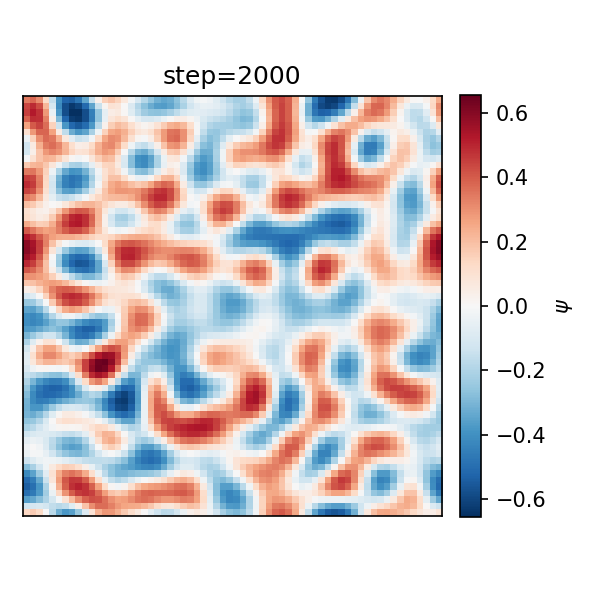
\includegraphics[width=0.32\textwidth]{figures/cahn-hilliard/early.png}\hfill
  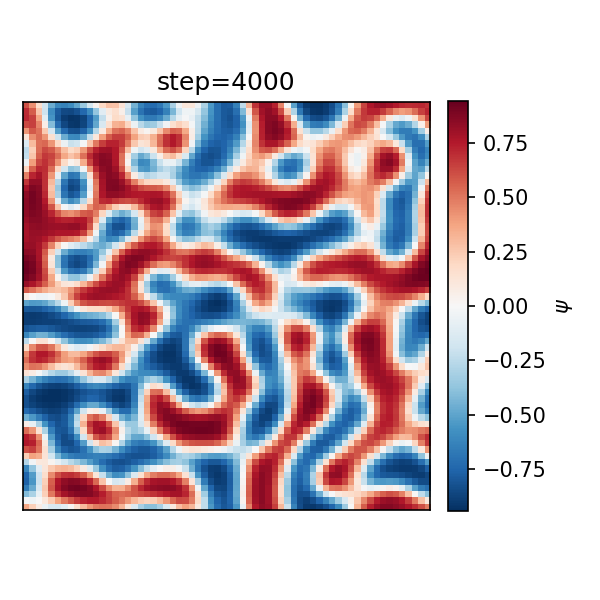
\includegraphics[width=0.32\textwidth]{figures/cahn-hilliard/mid.png}\hfill
  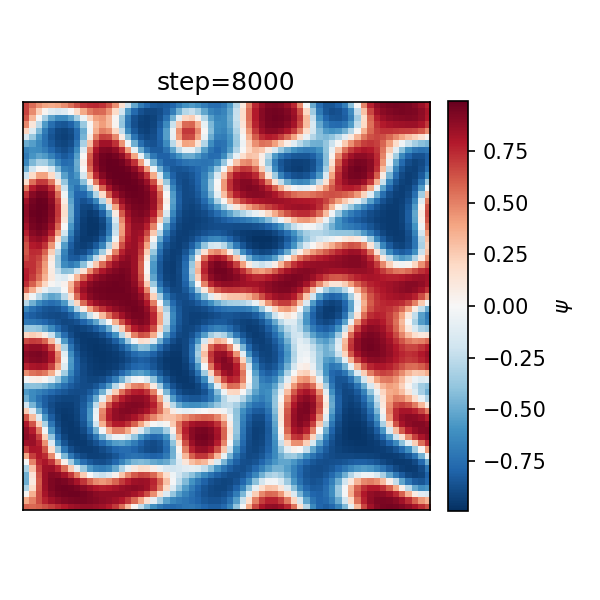
\includegraphics[width=0.32\textwidth]{figures/cahn-hilliard/late.png}
  \caption{$z$-midplane slices of $\psi$ from a $64^3$ Cahn--Hilliard
  run with $M=\kappa=1$, seed $42$, $\Delta x=1$, $\Delta t = 0.01$.
  Left ($t=20$): post-spinodal regime, $|\psi|$ has not yet saturated
  to the equilibrium amplitude. Center ($t=40$): bicontinuous
  two-phase pattern with sharp interfaces and $|\psi|\approx 1$. Right
  ($t=80$): coarsened domains, same amplitude. The reproduction of
  this textbook coarsening sequence is the qualitative-acceptance
  evidence for Phase 12.}
  \label{fig:ch-coarsening}
\end{figure}

The gradient energy
\(E_{\text{grad}} = \int |\nabla\psi|^2\,\dd V\) is a useful coarse
proxy for inverse domain size. In the default run it peaks near
\(t\approx 30\) (interfaces fully formed, smallest typical domains)
and decreases monotonically afterward. The Phase 12 acceptance test
\passthrough{\lstinline!CahnHilliardCoarseningRun.MonotoneCoarsening!}
locks in this property in CI on a smaller (24\(^3\), \(\kappa=0.5\))
budget-friendly run.

\subsection{What this does \emph{not} do}\label{phase12-not-do}

\begin{itemize}
\tightlist
\item
  \textbf{Implicit / IMEX time stepping.} The explicit
  \(\Delta t \sim h^4\) bound is brutal and grows worse with
  resolution. A semi-implicit treatment of the
  \(-M\kappa\nabla^4\psi\) term arrives in Phase 19 alongside the
  matrix-free linear-solver scaffolding.
\item
  \textbf{Non-periodic boundary conditions.} The demo runs purely on
  Phase 1's periodic \passthrough{\lstinline!IndexPolicy::Periodic!}.
  Dirichlet / Neumann at Phase 18 will let the same setup model a CH
  system with no-flux walls.
\item
  \textbf{\(R(t)\sim t^{1/3}\) quantitative scaling fit in CI.} The
  Phase 12 acceptance bar is qualitative (visual + monotone-coarsening
  programmatic check). A separately-runnable scaling benchmark could
  be added later.
\item
  \textbf{Vector- or tensor-valued CH.} Multi-component CH (model B
  for binary alloys with a multi-component order parameter) and model
  H (CH coupled to fluid flow) belong with Phase 13 / 14.
\end{itemize}

For the dispersion-relation derivation, the
\(\sigma(\mathbf k)\,\Delta t\le 2.7853\) RK4 stability argument, and
the rejected alternatives, see the ``Cahn--Hilliard demo'' chapter of
the Developer Note.
